%\documentclass[a4paper,11pt]{scrreprt}
%\documentclass[a4paper,15pt]{scrbook}
\documentclass[a4paper,11pt]{scrartcl}
%\documentclass[a4paper,13pt]{scrreprt}

\usepackage[T1]{fontenc}
\usepackage[utf8]{inputenc}
%\usepackage[latin9]{inputenc}
\usepackage{scrpage2}
\usepackage{titleref}
\usepackage[ngerman]{babel}
\usepackage{multicol}
\usepackage{lmodern}  
\usepackage{tabularx} 
\usepackage{graphicx}
\usepackage{blindtext}
\usepackage{microtype}
\usepackage{color}
\usepackage{colortbl}
\usepackage{framed} %umramen eines Bereiches
\usepackage[left=25mm,right=25mm,top=25mm,bottom=25mm]{geometry} % Standard
%\usepackage[left=20mm,right=20mm,top=25mm,bottom=30mm]{geometry}
%\usepackage[singlespacing]{setspace}
\usepackage[onehalfspacing]{setspace}
%\usepackage[doublespacing]{setspace}
\usepackage{verbatim}
\usepackage{listings}
%\usepackage[svgnames]{xcolor}
\usepackage{xcolor} 
\usepackage{setspace}
\usepackage{amsthm}
\usepackage{float}
\usepackage{pdfpages}
\usepackage{mdwlist}
\usepackage{prettyref}
\usepackage{multicol}
\usepackage[section]{minted}	
\usepackage{hyperref}

%%%%%% Beschriftung
\newcommand{\changefont}[3]{
\fontfamily{#1}\fontseries{#2}\fontshape{#3}\selectfont}


%%%%%% Farben 
\definecolor{hellgrau}{rgb}{0.95,0.95,0.95}
\definecolor{dunkelgrau}{rgb}{0.8,0.8,0.8}
\lstnewenvironment{beispiel}[3]{
    \lstset{language=#1, 
    numberbychapter=true,
    basicstyle=\ttfamily\small, 
    identifierstyle=\color{black}, 
    keywordstyle=\color{blue}, 
    stringstyle=\color{verde}, 
    commentstyle=\color{red}, 
   	breaklines=true, 
   	numbers=left,
   	label=#2,
   	caption=#3,
   	numberstyle=\small, 
   	frame=single}
   	\begingroup
   	\nopagebreak
   	}
   	{\endgroup}%  	   
   	

%%%%%%%%%%%%%%%%%%%%%%%%%%%%%%%%%%%%%%%%%%%%%%%%%%%%%%%%%%%%%%%%%%%%%%%%%%%%%%%
% \usepackage[section]{minted}
%  
% use "-shell-escape" as a new parameter for the command pdflatex
%
% \javacode{./folder/javacode.java}
% http://mirror.unl.edu/ctan/macros/latex/contrib/minted/minted.pdf
%%%%%%%%%%%%%%%%%%%%%%%%%%%%%%%%%%%%%%%%%%%%%%%%%%%%%%%%%%%%%%%%%%%%%%%%%%%%%%

%\newlength{\mintednumbersep}
%\AtBeginDocument{%
%  \sbox0{\tiny00}%
%  \setlength\mintednumbersep{\parindent}%
%  \addtolength\mintednumbersep{-\wd0}%
%}

\newmintedfile[javacode]{java}{
	bgcolor=mintedbackground,
	linenos=true,
	numberblanklines=true,
	numbersep=5pt,
	gobble=0,
	funcnamehighlighting=true,
	tabsize=4,
	obeytabs=false,
	mathescape=false
	samepage=true,
	showspaces=false,
	showtabs =false,
	texcl=false,
	fontsize=\scriptsize,
}
%%%%%%%%%%%%%%%%%%%%%%%%%%%%%%%%%%%%%%%%%%%%%%%%%%%%%%%%%%%%%%%%%%%%%%%%%%%%%%%
% \usepackage{listings}
%  
% \begin{listing}
%
% 
% https://en.wikibooks.org/wiki/LaTeX/Source_Code_Listings
%%%%%%%%%%%%%%%%%%%%%%%%%%%%%%%%%%%%%%%%%%%%%%%%%%%%%%%%%%%%%%%%%%%%%%%%%%%%%%



\lstset{numberbychapter=false, captionpos=b, caption=\lstname,frame=single,%
numbers=left, stepnumber=1, numbersep=2pt, xleftmargin=15pt, framexleftmargin=15pt,%
numberstyle=\tiny, tabsize=4, columns=fixed,%
basicstyle={\fontfamily{pcr}\selectfont\footnotesize},%
keywordstyle=\bfseries, commentstyle={\color[gray]{0.33}\itshape},%
stringstyle=\color[gray]{0.25}, breaklines, breakatwhitespace, breakautoindent}
\lstset{literate=
  {á}{{\'a}}1 {é}{{\'e}}1 {í}{{\'i}}1 {ó}{{\'o}}1 {ú}{{\'u}}1
  {Á}{{\'A}}1 {É}{{\'E}}1 {Í}{{\'I}}1 {Ó}{{\'O}}1 {Ú}{{\'U}}1
  {à}{{\`a}}1 {è}{{\`e}}1 {ì}{{\`i}}1 {ò}{{\`o}}1 {ù}{{\`u}}1
  {À}{{\`A}}1 {È}{{\'E}}1 {Ì}{{\`I}}1 {Ò}{{\`O}}1 {Ù}{{\`U}}1
  {ä}{{\"a}}1 {ë}{{\"e}}1 {ï}{{\"i}}1 {ö}{{\"o}}1 {ü}{{\"u}}1
  {Ä}{{\"A}}1 {Ë}{{\"E}}1 {Ï}{{\"I}}1 {Ö}{{\"O}}1 {Ü}{{\"U}}1
  {â}{{\^a}}1 {ê}{{\^e}}1 {î}{{\^i}}1 {ô}{{\^o}}1 {û}{{\^u}}1
  {Â}{{\^A}}1 {Ê}{{\^E}}1 {Î}{{\^I}}1 {Ô}{{\^O}}1 {Û}{{\^U}}1
  {œ}{{\oe}}1 {Œ}{{\OE}}1 {æ}{{\ae}}1 {Æ}{{\AE}}1 {ß}{{\ss}}1
  {ç}{{\c c}}1 {Ç}{{\c C}}1 {ø}{{\o}}1 {å}{{\r a}}1 {Å}{{\r A}}1
  {€}{{\EUR}}1 {£}{{\pounds}}1
}	
	
\begin{document}
%-------------------------------------
% Titelseite 
\thispagestyle{empty}
\begin{center}
	
\includegraphics[scale=.5]{./fau}\\
	\vspace*{2cm}
	\Large
	\textbf{Fakultät}\\
	\textbf{Informatik}\\
	\vspace*{2cm}
	\Huge
	\textbf{Design Patterns und Anti-Patterns}\\
	\vspace*{0.5cm}
	\large
	über das Thema\\
	\vspace*{1cm}
	\textbf{Verhaltensmuster: Visitor-, Command- und Observer-Pattern}\\
	\vspace*{2cm}
	
	\vfill
	\normalsize
	\newcolumntype{x}[1]{>{\raggedleft\arraybackslash\hspace{0pt}}p{#1}}
	\begin{tabular}{x{6cm}p{7.5cm}}
		\rule{0mm}{5ex}\textbf{Autor:} & Johannes Pfann\newline johannes.pfann@fau.de \\ 
		\rule{0mm}{5ex}\textbf{Abgabedatum:} & 08.06.2016 \\ 
	\end{tabular} 
\end{center}
\pagebreak
%-------------------------------------

%-------------------------------------
% Verzeichnisse  
\tableofcontents % Inhaltsverzeichnis
\pagebreak
%\listoffigures % Abbildungsverzeichnis 
%\listoftables % Tabellenverzeichnis 
%-------------------------------------

%-------------------------------------
% Textkörper
%\chapter{Einleitung}
%Einleitung

\subsection{Verhaltensmuster}

asdfasdf

%\chapter{Observer}
\section{Observer}
\glqq Definiere eine 1-zu-n-Abhängigkeit zwischen Objekten, so dass die Änderung des Zustands eines Objekts dazu führt, das alle abhängigen Objekte benachrichtigt und automatisch aktualisiert werden. \grqq 
\subsection{Beschreibung}
Das Observer-Pattern definiert durch die Interfaces \texttt{Subject} und \texttt{Observer} zwei Rollen denen unterschiedliche Aufgaben zugesprochen werden. Die Rolle Subject benachrichtigt die Rolle Observer, wobei diese sich um die Verarbeitung der Benachrichtigung kümmern muss. In der Regel besteht zwischen den zwei Rollen eine 1-zu-n-Abhängigkeit, sodass mehrere Observer von einem Subject benachrichtigt werden.
Damit das jeweilige Subject die einzelnen Observer kennen und benachrichtigen können, fordert die Rolle Subject die Implementierung zweier Methoden \texttt{attach(Obsever}, zum Anmelden  und eine \texttt{detach(Observer)} zum Abmelden eines Observers.
Die Rolle Observer hingegen definiert eine Methode \texttt{update(Object)} die zur Aktualisierung eines Observers von einem Subject aufgerufen wird, um diesen zu benachrichtigen.
In Abbildung \ref{observerdiagramm} sieht man ein UML-Diagramm mit den zwei Interfaces Subject und Observer. Die beiden konkreten Klassen \texttt{ConreteSubject} und \texttt{ConreteObserver} implementieren diese zwei Interfaces. Das ConcreteSubject muss neben der Implementierung der drei Methoden attach, detach und notifyObservers auch eine Collection zum Speichern der angemeldeten Observer beinhalten. Ein konkreter Observer muss hingegen nur die Methode update implementieren um auf eine Benachrichtigung entsprechend zu reagieren.

\begin{figure}[h!]
\centering
\includegraphics[width=0.7\textwidth]{./paper/observer/observer}
\caption{UML-Darstellung eines Observer-Pattern.}
\label{observerdiagramm}
\end{figure} 

\subsection{Beispiel}
Das Beispielszenario behandelt eine Arbeitsvermittlung deren Softwaresystem mit dem  Observer-Pattern umgesetzt wird. In dem Softwaresystem gibt es eine zentrale Komponente, das JobCenter, welches in regelmäßigen Abständen neue Stellenauschreibungen von externen Arbeitgebern mitgeteilt bekommt. Diese werden auf der Homepage, sowie auf Monitoren in der Arbeitsvermittlung aufgelistet. Bei einer neuen Stellenausschreibung soll das Jobcenter selbständig alle abhängigen Komponenten, wie Homepage und Monitore benachrichtigen, sodass diese sich aktualisieren können.
Für dieses Szenario nimmt das Jobcenter  die Rolle Subjects ein und die Homepage und die Monitore die Rolle Observer. Nachfolgend in Listing \ref{observer_observer_interface} und \ref{observer_subject_interface} sind diese zwei Rollen als Interfaces umgesetzt.
Das Subject definiert neben der Methode \texttt{notifyObsevers()}, zum benachrichtigen aller angemeldeten Observer eine Methode \texttt{attach(Observer)} und \texttt{detach(Observer)} zum An- und Abmelden eines Observers. Das Interface Observer muss hingegen nur zum aktualisieren einer Stellenausschreibung, eine Methode \texttt{update(Offer)} bereitstellen. Der Parameter \texttt{Offer} symbolisiert eine solche Stellenausschreibung, die über die genannte Update-Methode übergeben wird.


\begin{listing}[h!]
   \centering
   \javacode{./resources/observer_Observer_Interface.java}
   \caption{Observer Interface}
    \label{observer_observer_interface}
\end{listing}     
 
\begin{listing}[h!]
   \centering
   \javacode{./resources/observer_Subject_Interface.java}
   \caption{Subject Interface}
    \label{observer_subject_interface}
\end{listing}  
          
  
Im zweiten Schritt wird dann die Klasse JobCenter (siehe Listing \ref{observer_jobcenter}) implementiert, die von dem Interface Subject erbt und somit die Methoden \texttt{attach(Observer aObserver}, \texttt{detach(Observer aObserver)} und \texttt{notifyObservers()} umsetzt. Zusätzlich initialisiert das Subject eine Collection um die übergebenen Observer über die Attach-Methode zu speichern. Mit der Detach-Methode wird ein Obsever der Collection entfernt. Beim Aufruf der NotifyObserver-Methode wird dieser eine Stellenausschreibung übergeben, die allen gespeicherten Observern über die Update-Methode übergeben wird. 
Nennenswert ist,dass das die Klasse JobCenter an dieser Stelle nur das Interface Observer kennt und durch die Iteration ausnahmslos alle Observer benachrichtigt werden.

\begin{listing}[h!]
   \centering
   \javacode{./resources/observer_Arbeitsvermittlung.java}
   \caption{Jobcenter}
    \label{observer_jobcenter}
\end{listing} 

Als letztes betrachten wir die Klasse \texttt{Homepage} (siehe Listing \ref{observer_client}). Diese übernimmt die Rolle des Observers indem sie von dem Interface \texttt{Observer} erbt und die Methode \texttt{update(Offer aOffer)} implementiert. 

\begin{listing}[h!]
   \centering
   \javacode{./resources/observer_Klient.java}
   \caption{Observer - Homepage}
    \label{observer_client}
\end{listing}

In Abbildung \ref{observer_sequenz} wird der Ablauf eines solchen Szenarios anhand eines Sequenzdiagramm dargestellt. Zunächst melden sich die Observer \texttt{Homepage} und \texttt{Monitor} am Jobcenter an. Danach wird das JobCenter aktualisiert und alle angemeldeten Observer benachrichtigt, damit diese sich selbständig aktualisieren können.

\begin{figure}[h!]
\centering
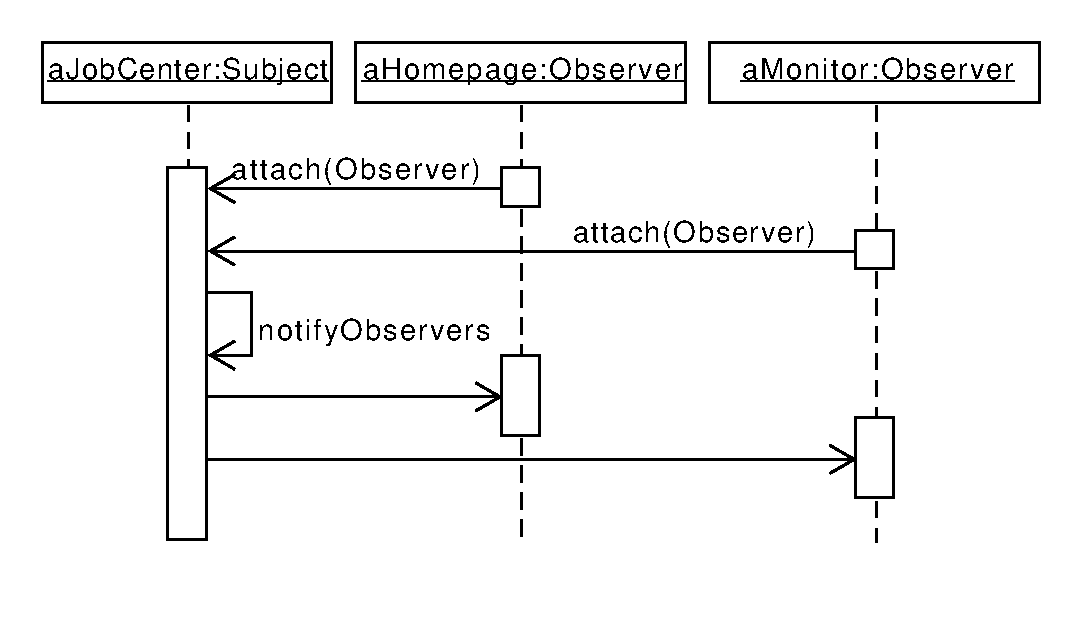
\includegraphics[width=0.7\textwidth]{./paper/observer/observer_sequenz}
\caption{Sequenzdiagramm mit dem Ablauf von JobCenter und desssen Clients}
\label{observer_sequenz}
\end{figure} 
\subsection{Implementierungsmöglichkeiten}
\section{Implementierung}
Für das Observer-Pattern gibt es mehrere Implementierungsmöglichkeiten. In Abschnitt 1.1 ... 


\paragraph{Push- oder Pull-Model} Bei den beiden Modellen werden die Unterschiedlichen Arten der Übertragung der Daten betrachtet. Bei dem Push-Model wird bei der Benachrichtigung ein oder mehrere Parameter übertragen. In unserem Fall muss das UML-Diagramm in Abbildung \ref{observerdiagramm} angepasst werden. Die Methode \texttt{aktualisieren()} benötigt einen zusätzlichen Parameter. Dieser wird dann bei dem Objekt \texttt{KonkretesSubjekt} beim Aufruf der Beobachter übergeben. Der Nachteil dieser Variante ist, das im Extremfall mehrere Parameter übergeben werden, jedoch nicht von jeden Observer benötigt werden. Oder ein neuer Beobachter benötrigt andere Daten wodurch man das Interface \texttt{Beobachter} und das Objekt \texttt{KonkretesSubjekt} anpassen muss.
Die Pull Methode verfolgt einen anderen Ansatz. Hier werden keine Daten als Parameter übergeben sondern die Beobachter greifen direkt nach einer Benachrichtigung auf die Instanz \texttt{KonkretesSubjekt} zu um die Daten zu erhalten. Der Nachteil dieser Variante ist, das die einzelnen Beobachter das Subjekt kennen müssen.

\paragraph{Lagerung der Beobachter} Hintegrund ist folgendes Szenario: Es gibt viele Subjekts und einige Beobachter. Die Subjekts müssen jetzt alle die Instanzen der jeweiligen Beobachter speichern. Um sich diesen Speicher zu ersparen, könnte man die Auflistung aller Beobachter in einer externen Datenstruktur bzw. Objekt lagern.

\paragraph{Beobachter beobachtet mehr als ein Subjekt} Für diesen Fall wird der Beobachter benachrichtigt und kann nicht wissen von welchem Objekt er aufgerufen wird. Abhilfe kann geschaffen werden, indem das konkrete Subjekt seine Instance beim Aufruf übermittelt, sodass der Beobachter eine Fallunterscheidung durchführen kann.

\paragraph{Ausführung des Updates} Das Anstoßen der Benachrichtigungen kann entweder vom Client als auch vom konkreten Subjekt durchgeführt werden. Der Vorteil dies dem Konkretem Subjekt zu überlassen ist die Vermeidung von Fehlern, indem der Client keine Benachrichtigung triggert. Falls die Verantwortung dem Client überlassen wird, kann dieser jedoch besser das Update nach Notwendigkeit steuern.

\paragraph{Aufräumen der Instansen} Es sollte Beachtet werden, das wenn ein Beobachter sich vom konkreten Objekt entfernt, auch die Instanz des konkreten SUbjekt aufräumt. 

\paragraph{Vor dem Benachrichtigen das Subjekt zuerst updaten} Bei der Implementierung des konkreten Subjekts sollte beachtet werden, vor der Benachrichtigung der Beobachter, zuerst das Subjekt zu aktualisieren. Gerade bei vererbten Methoden besteht Gefahr eines solchen Szenario.

\paragraph{Erweiterung der Benachrichtigung für ein bestimmtes Interesse} In bestimmten Fällen kann es sein, das ein Beobachter nur auf bestimmte Events benachrichtigt werden möchte. In diesem Fall bietet sich an,  die Methode \texttt{registriere()} um einen weiteren Parameter zu erweitern, damit der Beobachter dadurch das Interesse auf ein bestimmtes Event signalisieren kann.

\paragraph{Auslagerung der Verwaltung der Beobachter} Wenn die Beziehung zwischen den konkreten Subjekten und den Beobachtern zu komplex wird, empfiel sich die Verwaltung dieser auszulagern. In der Literatur wird von einem ChangeManager gesprochen. Dieser regelt folgende Gebiete: Das Mapping zwischen den Subjekten und den Beobachtern. Definiert spezielle Updatestrategien. Übernimmt die Benachrichtigung eines konkreten Subjekts für dessen Beobachter.

\paragraph{Subjekt als Interface oder Abstrakte Klasse} Das Subjekt kann ein Interface oder als abstrakte klasse implementiert sein. Der Nachteil bei einer abstrakten Klasse ist, dass nicht auf verschiedene konkrete Subjekts eingegangen werden kann. Jedoch erhöht sich der PRogrammieraufwand durch die wiederholte Implementierung des Selben Codes.



\subsection{Fazit}
\subsubsection{Vorteile}
\begin{itemize}
\item Wiederverwendbarkeit: Die Aufteilung von Beobachter und Subjekt sind Rollenbasiert. Ein Objekt kann sowohl ein Subjekt als auch ein Beobachter sein.
\item Abstrakte Kopplung von Beobachter und Subjekt: Das Subjekt kennt keinen konkreten Beobachter.  
\item Es muss im Voraus nicht bekannt sein, wie viele abhängige Objekte sich zur Laufzeit registrieren, und welche das sind.
\end{itemize}
\subsubsection{Nachteile}
\begin{itemize}
\item In manchen Fällen kann das Observer-Pattern allerdings zu Problemen führen. Beispielsweise könnte es zu Situationen kommen, dass mehrere Observer gleichzeitig Subjects von weiteren Observer sind usw. Die Komplexität steigt schenll bei solchen Sytemen und gerade bei der Fehlersuche kann dadurch erschwert werden.
\item Außerdem besteht die Gefahr von zyklischen Abhängigkeiten. Ein Subject kann durch komplexe Verkettungen gleichzeitig auch ein Observer dieser Abhängigkeitskette sein, sodass eine Benachrichtigung zu einer eigenen Aktualisierung führt, die wiederum  eine Benachrichtigung auslöst.
\end{itemize}


%\chapter{Command}
\section{Command}
\section{Definition}
\glqq Kapselung eines Requests als Objekt, um so die Parametrisierung von Clients mit verschiedenen Requests, Warteschlangen- oder Logging-Operationen sowie das Rückgängigmachen von Operationen zu ermöglichen.\grqq
\subsection{Beschreibung}
Das Ziel des Command-Pattern ist, den Requests und Receiver von dem Invoker auszulagern um diese flexibel austauschbar zu gestalten. Hierzu wird eine zusätzliche Schicht eingeführt, nämlich das Command-Objekt. In einem  Szenario ohne dem Command-Pattern, würde der Invoker den Receiver als Objekt kennen um darauf dessen Methoden aufzurufen. Dadurch ergibt sich allerdings, das der Receiver an den Invoker gebunden ist. Um das  Problem zu lösen, führt man auf der Seite des Invokers eine Schnittstelle, \texttt{Command} ein, die eine Methode \texttt{execute()} besitzt. Auf der andere Seite erstellt man ein konkretes Command, das von dieser Schnittstelle erbt und gleichzeitig den Receiver kennt, um dort diesen zu verwenden. Der Invoker muss also nur ein passendes Command-Objekt erhalten und  dessen Methode \texttt{execute()} aufrufen. Die konkrete Durchführung dieser Methode wird  dann in dem konkreten Command-Ojbekt behandelt. Abbildung \ref{commanddiagramm} zeigt ein UML-Diagramm für das Command-Pattern.


\begin{figure}[htbp]
\centering
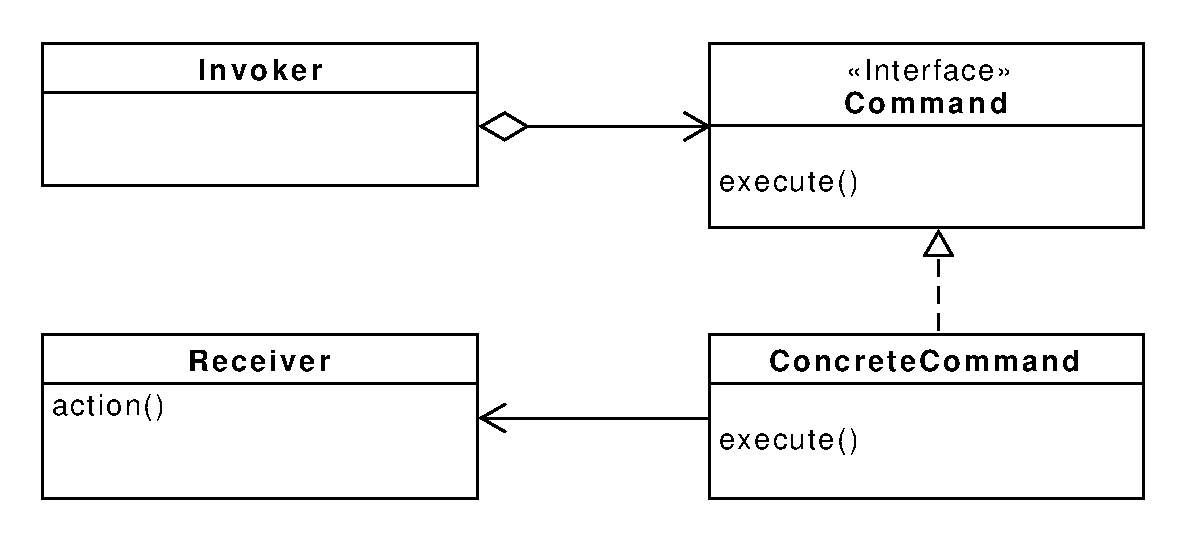
\includegraphics[width=0.7\textwidth]{./paper/command/command}
\caption{UML-Darstellung von dem Command-Pattern.}
\label{commanddiagramm}
\end{figure} 
\subsection{Beispiel}
Als  Beispieszenario wird  ein Logistikunternehmen das verschiedene Pakete versendet gewählt. Bei der Übermittlung von unterschiedlichen Paketen zu unterschiedlichen Empfängern müssen verschiedene Schritte getätigt werden. Außerdem können sich durch neue Richtlinien Arbeitsschritte ändern. 
Durch eine zusätzliche Schicht trennen wir das Vorhaben, ein Paket zu versenden von den tatächlichen Schritten, die es benötigt um ein Paket zu versenden. 
Als erstes konstruieren wir eine Schnittstelle \texttt{Command}. Dieser geben wir eine Methode \texttt{execute} mit dem Parameter Paket. 

\begin{beispiel}{java}{Command}{Command}
public interface Command {
    void execute(Paket aPaket);
}
\end{beispiel}

Danach erstellen wir das Logistikunternehmen als Objekt um von dort alle Arten von Paketen zu versenden. Welches Command-Objekt zum Ausführen der jeweiligen Schritte verwenden wird von außerhalb bestimmt.

\begin{beispiel}{java}{Logistikunternehmen}{InlandskundeSecureCommand}
public class Logistikunternehmen {
    Command mCommand = null;
    public Logistikunternehmen(Command aCommand){
        mCommand = aCommand;
    }
    public void versendePacket(Paket aPaket){
        mCommand.execute(aPaket);
    }
}
\end{beispiel}

Die erste Veriante um ein Paket zu versenden, ist das \texttt{InlandsKundenDefaultCommand}. Dieses kennt seinen Empfänger, nämlich den Inlandskunden und ruft auf diesem nur die Methode \texttt{empfangePaket} auf.

\begin{beispiel}{java}{InlandsKundeDefaultCommand}{InlandsKundeDefaultCommand}
public class InlandsKundeDefaultCommand implements Command{
    Inlandskunde mInlandskunde;
    public void execute(Paket aPaket) {
        mInlandskunde.empfangePaket(aPaket);
    }
}
\end{beispiel}

Die zweite Variante ist die sichere Übermittlung eines Paketes mit einer zusätzlichen Verpackung. Wieder kennt das Command-Objekt den Empfänger und ruft dessen Methode auf. Allerdings wird Logik in dem Command-Objekt behandelt indem das Paket zusätzlich verpackt wird.

\begin{beispiel}{java}{InlandskundeSecureCommand}{InlandskundeSecureCommand}
public class InlandskundeSecureCommand {
    Inlandskunde mInlandskunde;
    public void execute(Paket aPaket) {
        mInlandskunde.empfangePaket(verpackePacket(aPaket));
    }
}
\end{beispiel}


\subsection{Implementierungsmöglichkeiten}
Für das Command-Pattern ist aus der Sicht des Autors folgende drei Erweiterungsmöglichkeiten des Command-Patterns entscheident. Alle drei stammen aus [GoF]. 

\paragraph{Erweiterung durch eine Undo-Funktion} Da jetzt jeder Befehl bzw. Aktion in einem Objekt gekapselt ist, kann man sehr einfach diese in einer Liste oder ähnlichem Lagern. Mit dieser Erkenntnis könnte man auf diese Art eine Undo-Funktion realisieren, die alle getätigten Befehle zurücknimmt um zum Ausgangszustand zurückzukommen. Man könnte hierfür auch das Command-Objekt derart erweitern, dass zusätzliche Informationen

\paragraph{Aufgaben des Command-Objekts} Die Frage die man sich stellen sollte ist: Wie intelligent soll ein Command-Objekt sein. Einerseits kann man alle aufgaben an den Receiver deligieren. Das andere Extrem muss das Command-Objekt nichts von dem Receiver kennen und implementiert die komplette Logik.

\paragraph{Makro-Befehle} Denkbar ist auch, mehrere Receiver an das Command-Objekt zu geben um so mehrere Aktionen durchführen zu können.



\subsection{Fazit}
\subsubsection{Vorteile}
\begin{itemize}
\item Entkopplung von Befehl und
Ausführung.
\item Hohe Flexibilität durch
Austauschbarkeit
\end{itemize}

\subsubsection{Nachteile}
\begin{itemize}
\item Da jede neue Ausführung eines Commands in eine neue Klasse implementiert werden muss, führt das zu einer hohen Anzahl der Klassen.
\end{itemize}


%\chapter{Visitor}
\section{Visitor}
\glqq Das Visitor Pattern ermöglicht es, neue Operationen auf den Elementen einer Struktur zu definieren, ohne die Elemente selbst anzupassen.\grqq (vgl. \cite{EIST06})
\subsection{Beschreibung}

Das Ziel des Visitor-Pattern ist, die Operationen auf Elemente in einer Objektstruktur außerhalb dieser Objektstruktur zu lagern um diese beliebig auszuwechseln.
Die Voraussetzung für jedes Element dieser Objektstruktur ist ein Interface \texttt{Element}, welches eine Methode \texttt{accept(Visitor)} erfordert. Dabei repräsentiert das übergebene Objekt \texttt{Visitor} die Operationen, die auf dieses Element angewendet werden sollen. Der Visitor selbst ist auch ein Interface. Das Interface muss für jeden Typ Element eine eigene Methode implementieren, die für die Bearbeitung der jeweiligen Elemente verantwortlich sind. Das bedeutet für unser UML-Diagramm, mit den zwei verschiedenen Elementen \texttt{ElementA} und \texttt{ElementB}, das wir zwei Methoden \texttt{visitElementA(ElementA)} und \texttt{visitElementB(ElementB)} definieren müssen. 
Der Ablauf des Visitor-Pattern ist folgendermaßen: Zunächst wird einem Element ein konkretes Visitor-Objekt übergeben. Dieses Element ruft dann die für sich implementierte Visit-Methode auf und übergibt sich selbst dem Visitor. Der Visitor kann so auf das Element zugreifen und es bearbeiten.

\begin{figure}[htbp]
\centering
%\includegraphics[scale=.5]{./observer/observer}
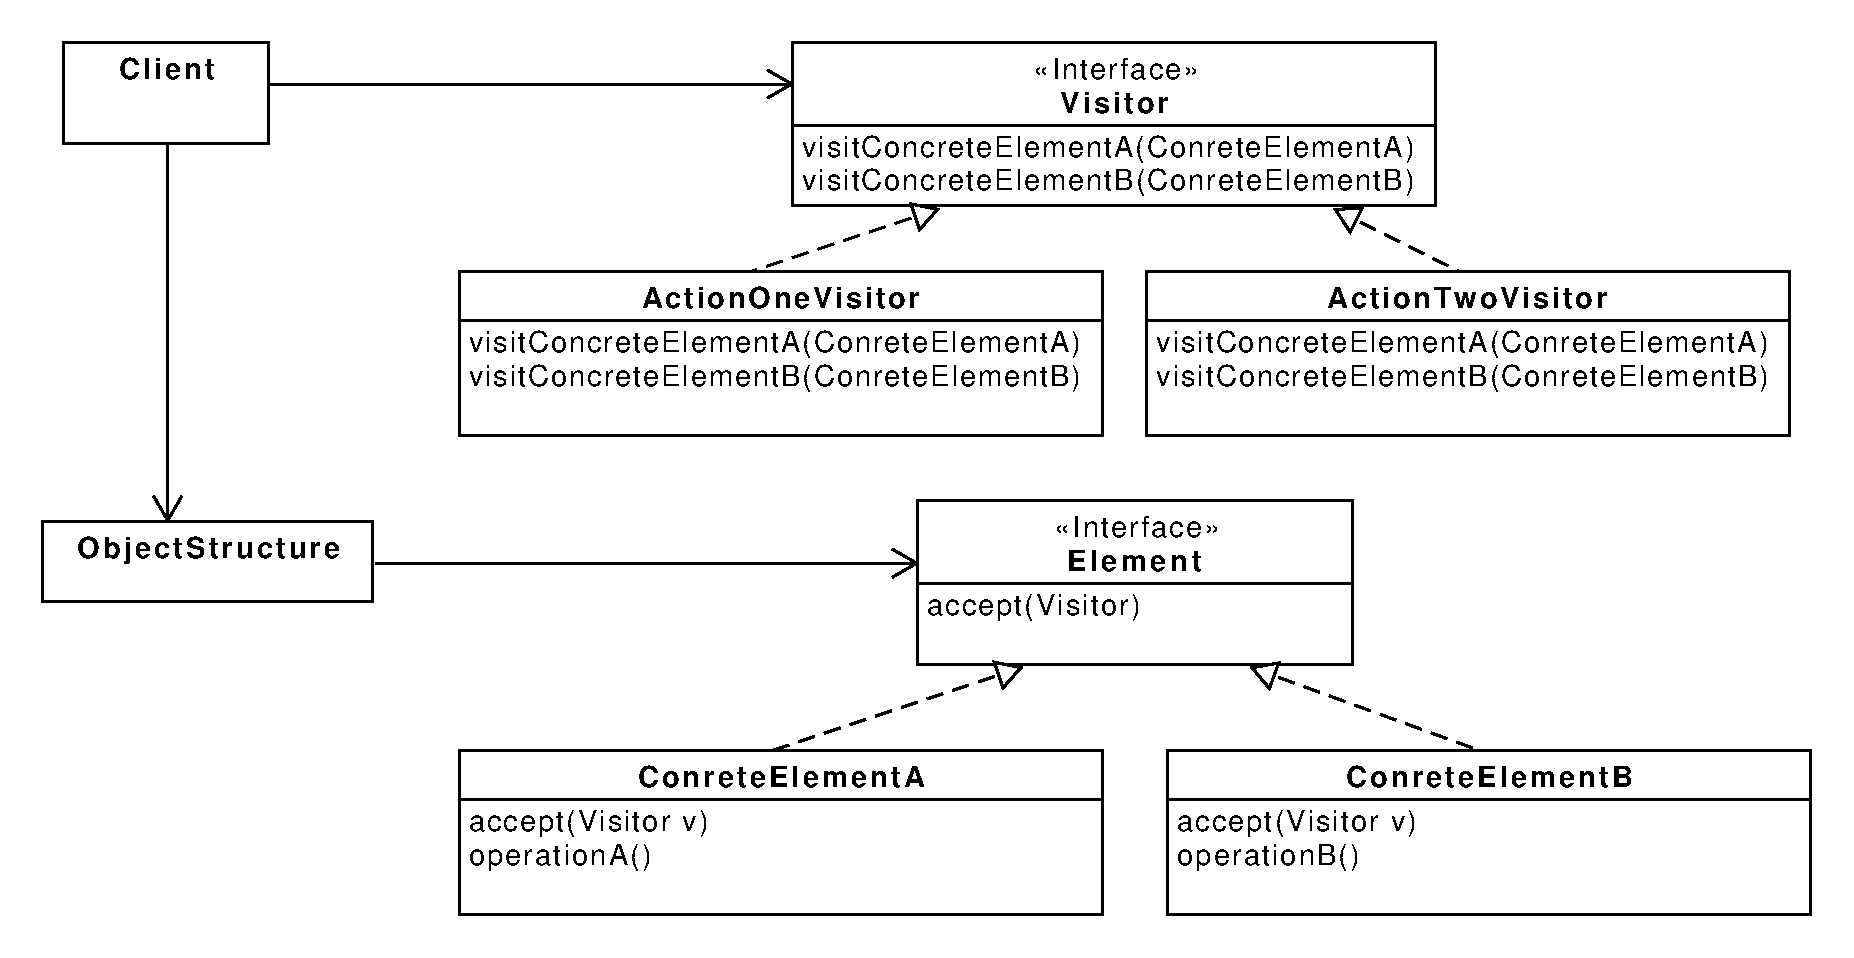
\includegraphics[width=0.7\textwidth]{./paper/visitor/visitor}
\caption{UML-Darstellung von dem Visitor-Pattern.}
\label{visitordiagramm}
\end{figure} 

\subsection{Implementierungsmöglichkeit}

Wer ist für die Traversierung der  Objektstruktur verantwortlich? Ein Visitor-Objekt muss jedes einzelne Element der Objektstruktur aufsuchen. Hierfür gibt es drei Implementierungsmöglichkeiten. 
\paragraph{Die Objektstruktur} Die Objektstruktur übernimmt die Zuständigkeit über all seine Elemente zu traversieren. Dieses geschieht oft mithilfe eines Composite Patterns, bei dem ein Element seine Kindelemente mit deren Mehtode \texttt{accept} aufruft und einen Vistor übergibt.
\paragraph{Der Iterator} Eine andere Möglichkeit ist ein interner oder externer Iterator. Dieser könnte bei dem Aufruf des nächsten Elements die Methode \texttt{accept} anstoßen.
\paragraph{Der Visitor} Die letzte der drei Varianten ist, die Traversierung den Visitor-Objekten zu überlassen. Der Nachteil dieser Variante ist , mehrfach den Traversierungscodein den verschiedenen Vistors zu haben. Hierfür könnte man allerdings eine abstrakte Klasse einführen, der den redundanten Code eliminiert. Der entscheidente Vorteil dieser VAriante ist, verschiedene Möglichkeiten der Traversierung durch die Objektstruktur anzubieten.




\subsection{Beispiel}

Um das Visitor-Pattern besser zu demonstrieren, wird dieses anhand des folgenden Beispiels erklärt. In einer Küche gibt es mehrere Sorten Gemüse. Die Variation dieser verschiedenen Sorten ist überschaubar und wird sich nicht mehr ändern. Allerdings ist unklar, welche Operationen auf diese Objekte angewendet werden und in Zukunft noch angewendet werden könnten. Um dieses zu berücksichtigen erstellen wir eine Objektstruktur und verlagern die Operationen auf dieses nicht in den Objekten selbst, sondern außerhalb. Hierfür erstellen wir zunächst ein Interface \texttt{Element} mit der Schnittstelle \texttt{accept(Visitor aVisitor}, der Objekte mit dem Interface \texttt{Vistor} entgegennehmen kann.  Methode.


\begin{listing}[h!]
   \centering
   \javacode{./resources/visitor_element_interface.java}
   \caption{Element Interface}
    \label{visitor_element_interface}
\end{listing}  


Dementsprechend benötigen wir ein Interface \texttt{Visitor} das die Methoden zum Besuchen der einzelnen VArianten der Elemente bereitstellt.

\begin{listing}[h!]
   \centering
   \javacode{./resources/visitor_visitor_interface.java}
   \caption{Visitor Interface}
    \label{visitor_visitor_interface}
\end{listing}  

 
Zunächst betrachten wir einen konkreten Visitor. Die erste Operation für alle Sorten bezieht sich auf das Waschen. Hierfür wird ein WaschenVisitor implementiert, der jeweils alle Methoden bereitstellt zum besuchen des jeweiligen Elements. 

\begin{listing}[h!]
   \centering
   \javacode{./resources/visitor_cleanvisitor.java}
   \caption{CleanVisitor}
    \label{visitor_cleanvisitor}
\end{listing}  


Nachfolgend betrachten wir nur das Element \texttt{Apfel}. In der visit-Methode wird ein Apfel übergeben, der dann auf diesem Element entsprechenden Operationen ausführt.
Diese Methode wird allerdings in der accept-Methode der Klasse \texttt{Apfel} aufgerufen. Die Methode \texttt{accept} ruft die Methode \texttt{visit} des aktuellen Visitors auf (in diesem Fall der WaschenVisitor) und übergibt sich selbst dieser


\begin{listing}[h!]
   \centering
   \javacode{./resources/visitor_potato.java}
   \caption{CleanVisitor}
    \label{visitor_potato}
\end{listing}  



\subsection{Fazit}
\subsubsection{Vorteile}
\begin{itemize}
\item Es können weitere Operationen hinzugefügt werden, ohne die Objektstruktur anzupassen.
\item Funktionalität kann so gezielt auf bestimmte Arten von Objekten eingesetzt werden.
\item Verwandte Operationen werden im Visitor zentral verwaltet.
\end{itemize}
\subsubsection{Nachteile}
\begin{itemize}

\item Problematisch ist, dass Elemente öffentliche Attribute und Methoden bereitstellen müssen zur Manipulation durch den Visitors. 
\item Das Hinzufügen von neuen Elementen ist mit der Änderung von allen Vistors verbunden.
\end{itemize}


%-------------------------------------
% Quellen / Glossar
%%%%%%%%%%%%%%%%%%%%%%%%%%%%%%%%%%%%%%%%%%%%%%%%%%%%%%%%%%%%%%%%%%%%%%%%%%%%%%%
%
%  http://www.weinelt.de/latex/thebibliography.html
%  \bibitem[Markierung]{Kennung}Quelle
%  \cite[Spezifikation]{Kennung}
%  \cite{GARR05}) kann auf die Quelle zugegriffen werden
%
%%%%%%%%%%%%%%%%%%%%%%%%%%%%%%%%%%%%%%%%%%%%%%%%%%%%%%%%%%%%%%%%%%%%%%%%%%%%%%%

\begin{thebibliography}{12cm}

\bibitem[GOF95]{GOF95} Erich Gamma, Richard Helm, Ralph E. Johnson, John Vlissides: Entwurfsmuster. Elemente wiederverwendbarer objektorientierter Software. Addison-Wesley, München 2004, ISBN 3-8273-2199-9.

\bibitem[EIST06]{EIST06} Karl Eilebrecht, Gernot Starke: Patterns Kompakt: Entwurfsmuster für effektive Softwareentwicklung Spektrum Akademischer Verlag, 4 Auflage 2006, ISBN 3-8274-1443-1

\bibitem[IN15]{IN15} Michael Inden: Der Weg zum Java-Profi: Konzepte und Techniken für die professionelle Java-Entwicklung, dpunkt.verlag,Heidelberg 2015, ISBN 978-86490-203-1

   

\end{thebibliography}

%-------------------------------------

\end{document}